
The aim of our bibliographic study using the systematic mapping methodology \cite{SM:Petersen:2008} is to (i) categorize and quantify the key contributions and the evolution of the research done on \textit{SLA-guided
data integration in a multi-cloud environment} and  (ii) discover open issues and limitations of existing works.    
Our study is guided by  three research questions:


\textit{\textbf{RQ1:} Which are the SLA measures that have been mostly
applied  in the cloud?} This question  identifies  the type of
properties used for characterizing and evaluating the services provided  by
different clouds. 
% It will also help to identify  the type of measures used for
% evaluating the properties and expressing them in service level agreements.      
 
\textit{\textbf{RQ2:}  How have published papers on data
 integration evolved towards cloud topics?} This question is devoted to identify the way  data integration problems addressed in the literature started  to include issues introduced by the cloud.

\textit{\textbf{RQ3:} In which way and in which  context has data integration  been linked to Quality of Service (QoS) measures in the literature?} The objective of this question is to understand which QoS measures have been used for evaluating data integration and to determine the conditions in which  specific measures are particularly used.

%--------------------------------------------------------------------------------------------------------------------------------------------
\subsection{Searching and screening  papers} \label{subsec:search}
%--------------------------------------------------------------------------------------------------------------------------------------------

According to our research questions and our expertise in data integration we chose a set of keywords to define a complex query to be used for retrieving papers from four target publication databases: IEEE~\footnote{http://ieeexplore.ieee.org/},
ACM~\footnote{http://dl.acm.org/}, Science Direct~\footnote{http://www.sciencedirect.com/} and
CiteSeerX~\footnote{http://citeseerx.ist.psu.edu/}. We used the following conjunctive and disjunctive general query which was completed with associated terms from a thesaurus and rewritten according to the expression rules of advanced queries in each database: 




\begin{center}
\textit{("Service level agreement"  AND ("Data integration" OR "Database
integration") AND ("Cloud" OR "Multi-cloud "))} \\
\end{center}
\medskip

% \begin{table}[!ht]
% \begin{center}
% \begin{tabular}{>{\centering\arraybackslash}p{2.5cm}|>{\centering\arraybackslash}p{2.5cm}|>{\centering\arraybackslash}p{2.5cm}|>{\centering\arraybackslash}p{2.5cm}}
% \toprule
% \textbf{Database} & \textbf{Amount} & \textbf{Included} & \textbf{Excluded} \\ 
% \hline \toprule
% \textbf{IEEE} & 658 & 56 & 602 \\ 
% \hline 
% \textbf{AMC} & 649 & 31 & 618	 \\ 
% \hline 
% \textbf{Science Direct} & 106 & 6 & 100 \\ 
% \hline  
% \textbf{CiteSeerX} & 419 & 21 & 398 \\ 
% \hline 
% \textit{Total} & 1832 & \textbf{114} & 1718 \\ 
% \bottomrule \hline
% \end{tabular} 
% \end{center}
% \caption{Number of papers retrieved in each scientific database}\label{table:pub}
% \end{table}

% We retrieved  a total of 1832 publications. According to the systematic mapping methodology, the initial collection was cleaned and filtered according to inclusion and exclusion criteria applied as filters when analyzing the titles and abstracts of the papers. 
% %(see table~\ref{table:criteria}).  
% In general, we only kept publications written in English, addressing SLA models
% and languages, quality measures, and/or (multi)-cloud topics related to data
% integration. As a result of the filtering process we excluded 1718 publications.
% The number of papers included for building the final collection were 114
% publications~\footnote{List of references available in:
% https://github.com/danielboni/DEXA-2015-Can-Data-Integration-Quality-be-Enhanced-on-Multi-cloud-using-SLA.git}.
  

We retrieved  a total of 1832 publications. As a result of the filtering process
proposed by the systematic mapping methodology~\cite{SM:Petersen:2008} we excluded 1718 publications.
The number of papers included for building the final collection were 114
publications~\footnote{List of references available in:
https://github.com/danielboni/DEXA-2015-Can-Data-Integration-Quality-be-Enhanced-on-Multi-cloud-using-SLA.git}.
  
% The columns \textit{Included} and \textit{Excluded} in Table~\ref{table:pub}
% summarize the number of papers per database that were included and excluded for
% building the final collection with 114 publications.

%--------------------------------------------------------------------------------------------------------------------------------------------
\subsection{Defining classification facets}
%--------------------------------------------------------------------------------------------------------------------------------------------

We analyzed the titles and abstracts of the  papers derived in the previous
phase using information retrieval techniques  to identify  frequent
 terms. We used these terms for proposing a classification scheme
consisting of three facets that group dimensions. The following lines define the facets and dimensions of the
classification scheme we propose. 
%  for studying SLA guided data integration
% in multi-cloud environments.
% We added two 
% facets for classifying the type of papers (e.g., position, survey, etc.) and the
% type of contributions (e.g., model, system, language, etc). 


%.  -   .  .  -   ..  -   ..  -   ..  -   ..  -   ..  -   ..  -   ..  -   ..  -   ..  -   ..  -   ..  -   ..  -   ..  -   ..  -   ..  -   ..  -   ..  -   ..  -   ..  -   ..  -   ..  -   ..  -   .  
\textbf{\textit{Data Integration Environment:}}  
%.  -   .  .  -   ..  -   ..  -   ..  -   ..  -   ..  -   ..  -   ..  -   ..  -   ..  -   ..  -   ..  -   ..  -   ..  -   ..  -   ..  -   ..  -   ..  -   ..  -   ..  -   ..  -   ..  -   ..  -   .  
This facet groups the dimensions that characterize the architectures used for delivering data integration services ({\em data warehouse} and  {\em federated database}) and  architectures used for deploying these services ({\em cloud} and {\em multi-cloud}).
%\begin{table}[h]
%\begin{center}
%\begin{tabular}{p{4cm}p{10cm}}
%\hline 
%\textbf{Dimension} & \textbf{Publication} \\ 
%\hline 
%Cloud & 
%\cite{106,110,105,107,108,109,068,070,072,113,073,074,075,076,077,078,079,081,082,083,085,087,088,089,090,094,095,096,097,098,099,100,102,103}\\ 
%\hline 
%Data Warehouse & \cite{066,114,091} \\ 
%\hline 
%Federated Database & \cite{071,089,112} \\ 
%\hline 
%Multi-cloud & \cite{012,071,093} \\ 
%\hline 
%\end{tabular}
%\end{center}
%\caption{Data Integration Environment facet}\label{table:dienviron}
%\end{table}

%\begin{table}[!h]
%\begin{center}
%\begin{tabular}{p{4cm}p{4cm}}
%\hline 
%\textbf{Dimension} & \textbf{Publication} \\ 
%\hline 
%Cloud & 34 \\ 
%\hline 
%Data Warehouse & 3 \\ 
%\hline 
%Federated Database & 3 \\ 
%\hline 
%Multi-cloud & 3 \\ 
%\hline 
%\end{tabular}
%\end{center}
%\caption{Data Integration Environment facet:  papers per dimension}\label{table:dienviron}
%\end{table}

%.  -   .  .  -   ..  -   ..  -   ..  -   ..  -   ..  -   ..  -   ..  -   ..  -   ..  -   ..  -   ..  -   ..  -   ..  -   ..  -   ..  -   ..  -   ..  -   ..  -   ..  -   ..  -   ..  -   ..  -   .  
\textbf{\textit{Data Integration Description:}}
%.  -   .  .  -   ..  -   ..  -   ..  -   ..  -   ..  -   ..  -   ..  -   ..  -   ..  -   ..  -   ..  -   ..  -   ..  -   ..  -   ..  -   ..  -   ..  -   ..  -   ..  -   ..  -   ..  -   ..  -   .  
 %As shown in table~\ref{table:didesc} 
 This facet groups the dimensions describing the approaches used for describing the databases content in order to  integrate them. Data integration can be done by using {\em meta-data, schema}, and {\em knowledge}.
%\begin{table}[h]
%\begin{center}
%\begin{tabular}{p{4cm}p{10cm}}
%\hline 
%\textbf{Dimension} & \textbf{Publication} \\ 
%\hline 
%Knowledge & \cite{012,083} \\ 
%\hline 
%Metadata & \cite{108,066,113} \\ 
%\hline 
%Schema & \cite{070,071,072,073,075,114,083,089,091,112,102} \\ 
%\hline 
%\end{tabular}
%\end{center}
%\caption{Data Integration Description facet}\label{table:didesc}
%\end{table}

%\begin{table}[!h]
%\begin{center}
%\begin{tabular}{p{4cm}p{4cm}}
%\hline 
%\textbf{Dimension} & \textbf{Publication} \\ 
%\hline 
%Knowledge & 2 \\ 
%\hline 
%Metadata & 3 \\ 
%\hline 
%Schema & 11 \\ 
%\hline 
%\end{tabular}
%\end{center}
%\caption{Data Integration Description facet: papers per dimension}\label{table:didesc}
%\end{table}

%.  -   .  .  -   ..  -   ..  -   ..  -   ..  -   ..  -   ..  -   ..  -   ..  -   ..  -   ..  -   ..  -   ..  -   ..  -   ..  -   ..  -   ..  -   ..  -   ..  -   ..  -   ..  -   ..  -   ..  -   .  
\textbf{\textit{Data Quality:}} 
%.  -   .  .  -   ..  -   ..  -   ..  -   ..  -   ..  -   ..  -   ..  -   ..  -   ..  -   ..  -   ..  -   ..  -   ..  -   ..  -   ..  -   ..  -   ..  -   ..  -   ..  -   ..  -   ..  -   ..  -   .  
%As shown in table~\ref{table:dq} 
This facet groups the dimensions  representing data quality measures. Measures can be related directly to data for instance {\em confidentiality, privacy, security, protection and provenance} and to the conditions in which data is integrated and delivered  (i.e., dimension {\em SLA}).

% Today, data integration has to do with  classic problems: (i) the approach used
% for providing a global integrated representation of different data collections
% described by the facet {\em data integration description} of our scheme.
% According to the dimensions of our classification, this can be done either by
% defining a schema (e.g., global and local as view approaches), by tagging data
% with meta-data or by associating them to knowledge (e.g. semantic Web
% approaches). (ii) The integration and the deployment architectures used for
% integrating data described by the facet {\em Data integration environment}.
% According to our classification scheme data can be integrated in {\em data
% warehouses} where there is the notion of one repository that stores and
% sometimes consolidates data stemming from different sources; or in a {\em
% federation} with a mediator aware of the content of different data sources and
% that can give global access to these distributed data. Finally data warehouses
% and database federations can be deployed on {\em cloud} and {\em multi-cloud}
% environments.               

The original vision of our classification scheme is that of adding the notion of {\em quality} to data integration represented by the facets {\em data quality} 
%that groups the measures used in SLAs; 
and  {\em SLA}.
%characterizing the way SLAs are expressed and associated to data integration (e.g., model, language). 
With these facets our classification scheme shows the aspects that must be considered when addressing data integration in the cloud  taking into account (i) the quality of data, (ii) the systems that integrate data and (iii) the quality warranties that a data consumer can expect expressed in SLAs.

% Facets and dimensions define the  scheme we used for  classifying the papers  according to dimensions. 
% Each paper can be classified into one or several dimensions of each facet. This is described in the following section.

%------------------------------------------------------------------------------- %
\subsection{Quantitative Analysis}\label{sec:qanalysis}
%--------------------------------------------------------------------------------% 

This section discusses the quantitative analysis  presented in bubble charts that combine different facets. 
In order to observe the evolution of the publication trends we defined a time screen between the years 1998 and 2014 (see Figure \ref{fig:pubperyear}). SLA has emerged when Cloud issues started to be addressed around 2009. The number of publications has increased as cloud infrastructures have become more popular and accessible. It seems  that data integration is an open issue when it is combined with SLA and cloud trends. Less recent papers seem to be devoted to the way data is described under schemata or knowledge representation strategies. This could be due to the fact that these strategies are consolidated today and  to the emergence of NoSQL approaches with their schema-less philosophy \cite{sadalage2012nosql}. 

\begin{figure}[ht!]
\centering
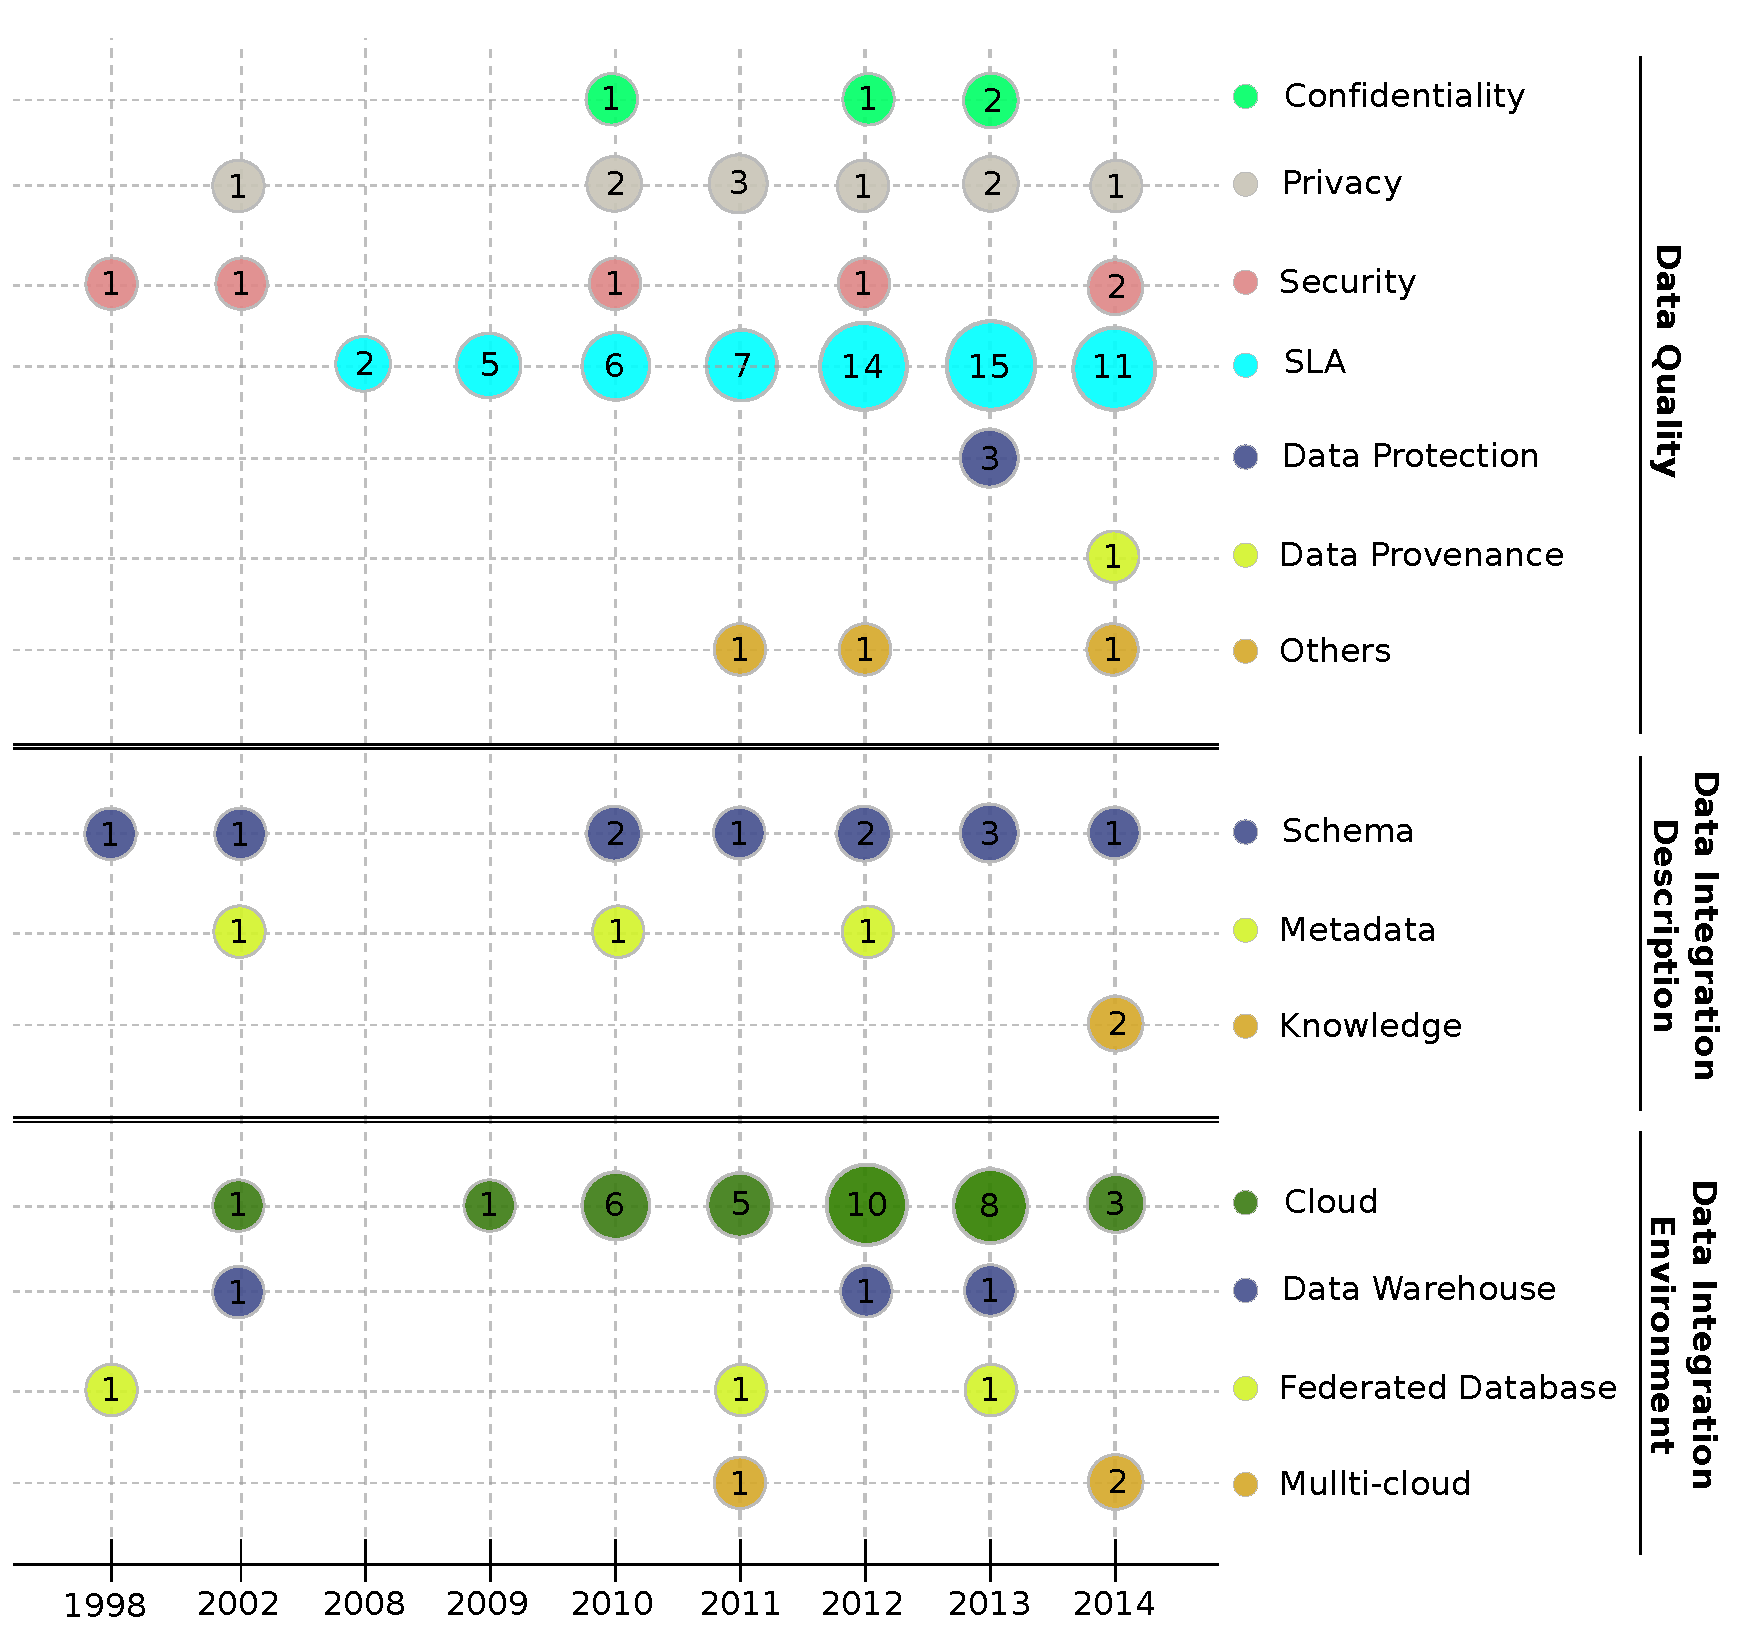
\includegraphics[scale=0.33]{figs/bubble-charts/PublicationsPerYear.pdf} 
\caption{Publications Per Year}\label{fig:pubperyear}
\end{figure}

We combined facets for answering the research questions proposed for guiding our
study. The following lines discuss the answers.

%Our analysis presents the frequencies of publications for
%the choosen facets. The charts show the aggregated view of the number of papers 
%considering the facets. This approach will help answer the three research
%questions more objectively.

 
%  . .  .  . .  .  . .  .  . .  .  . .  .  . .  .  . .  .  . .  .  . .  .  . .  .  . .  .  . .  .  . .  .  . .  .  . .  .  . .  .  . .  .  . .  .  . .  .  . .  .  . .  .  . .  .
\textbf{\textit{RQ1: Which are the SLA measures that have been mostly applied 
in the cloud?}}
%  . .  .  . .  .  . .  .  . .  .  . .  .  . .  .  . .  .  . .  .  . .  .  . .  .  . .  .  . .  .  . .  .  . .  .  . .  .  . .  .  . .  .  . .  .  . .  .  . .  .  . .  .  . .  .


The facets SLA expression, data integration description and contribution give elements for determining which SLA measures have been applied to the cloud (Figure~\ref{fig:facet1}). 
The resulting bubble chart shows that most contributions propose SLA models and that  \textit{privacy}
and \textit{security} (11 papers - 9.65\%) are the most popular measures considered by SLA models for the cloud. These measures concern the network, information, data protection and confidentiality in the cloud. Most contributions propose SLA models (53 papers - 46.49\%)  but some languages (8 papers - 7.02\%) have also emerged. {\em Data provenance} is also a measure that emerges but only in papers dealing with multi-cloud environments. Data integration is merely addressed by using schemata (12 papers - 10.53\%)  and meta-data (4 papers - 3.51\%) particularly through models (34 papers - 29.82\%) and tools (25 papers - 21.93\%). Still, some works propose surveys (8 papers - 7.02\%).
 
\begin{figure}[ht!]
\centering
%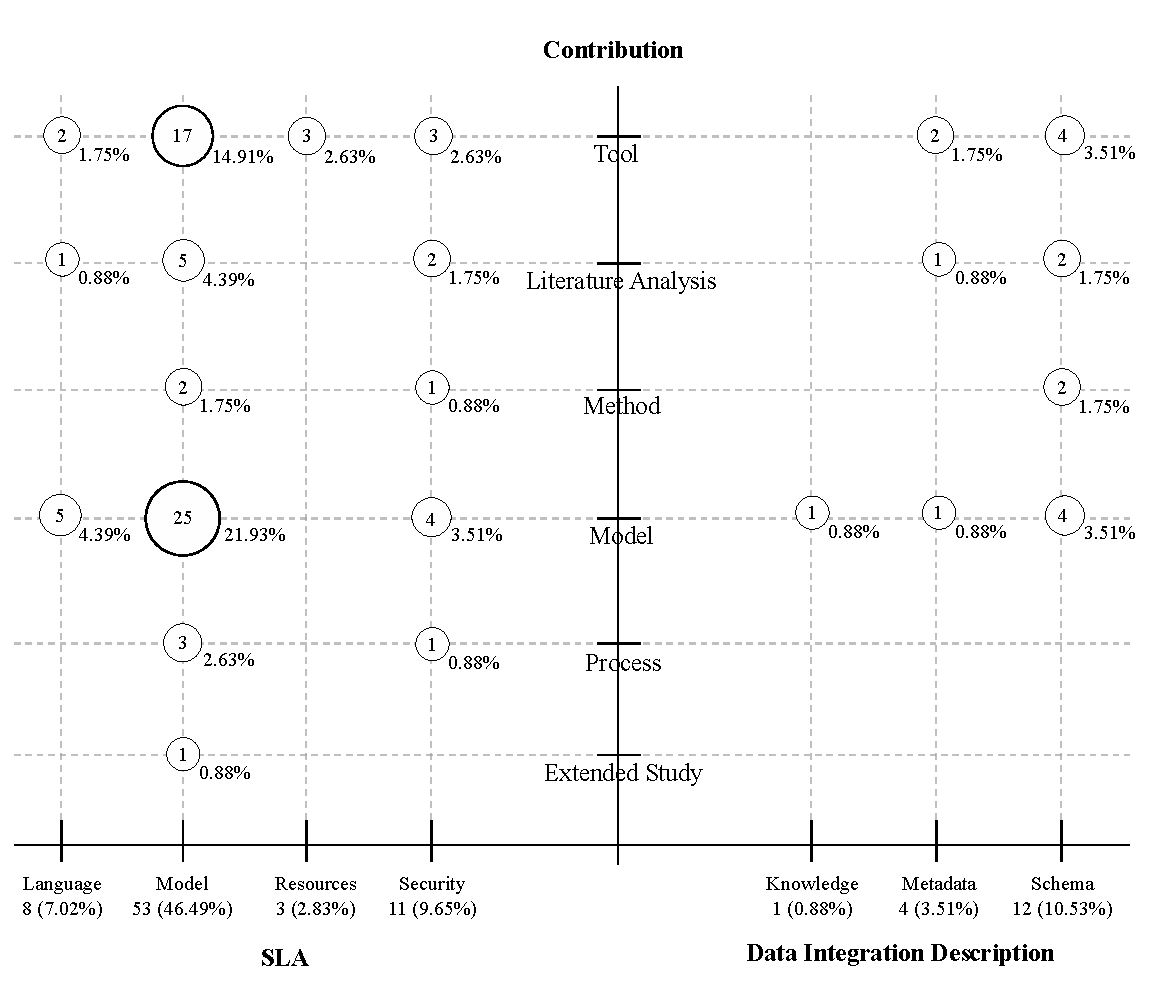
\includegraphics[scale=0.45]{figs/bubble-charts/Contribution-SLA-DIdescription.pdf}
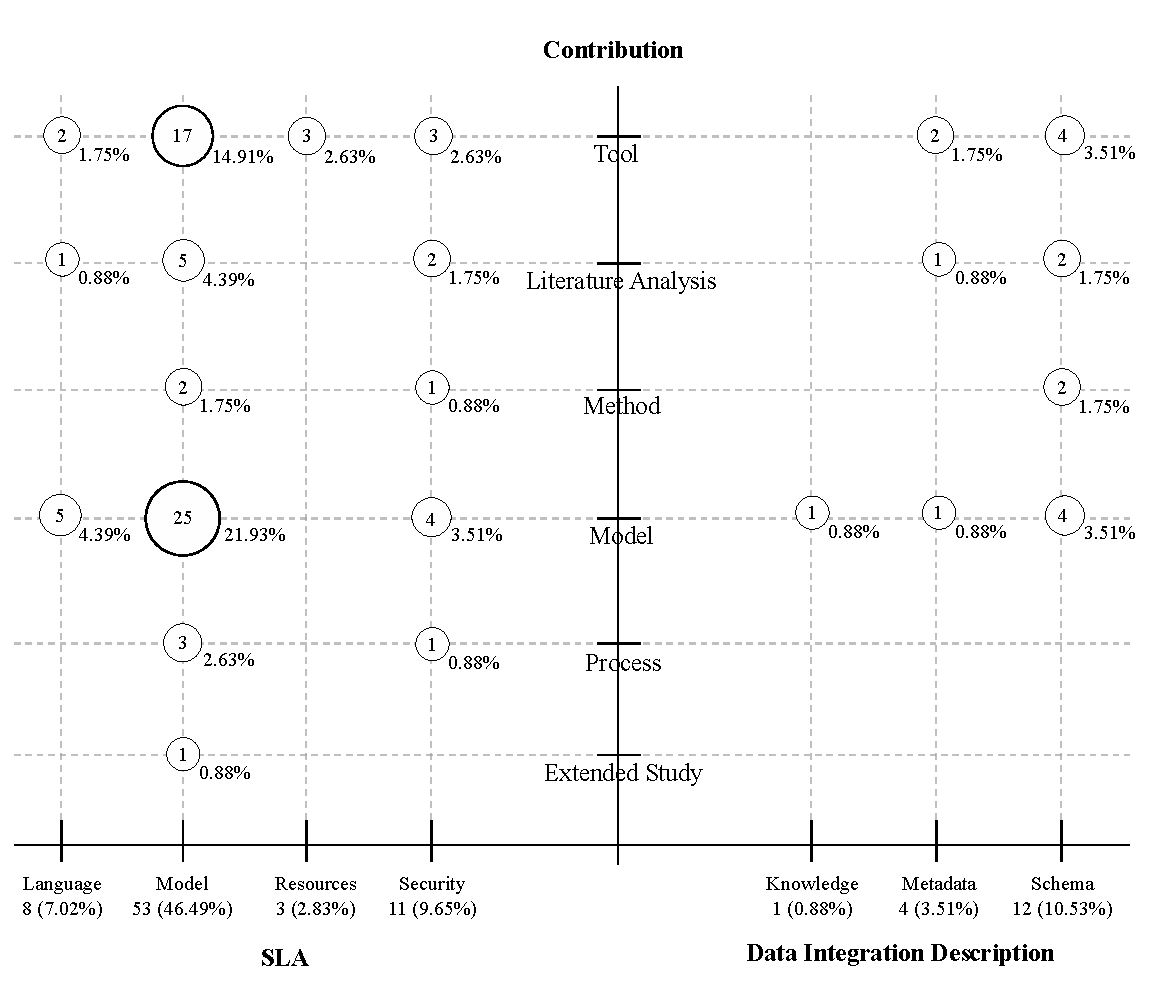
\includegraphics[width=0.75\textwidth]{figs/bubble-charts/Contribution-SLA-DIdescription.pdf}
  
\caption{Facets Contribution, SLA and Data Integration Description}\label{fig:facet1}
\end{figure} 
%The most used type of environment is \textit{cloud}, followed by \textit{data
%warehouse, multi-cloud} and \textit{federated database}. Looking to the figure
%you can alse note that models for SLA have been the focus in the papers (53 appearances - 46.49\%) followed by Security (11 appearances - 9.65\%), Language 
%(8 appearances - 7.02\%) and Resources (3 appearances - 22.83\%).
%Analyzing the figure is also possible to observe that Model (34 appearances - 29.82\%) and 
%Tool (25 appearances - 21.93\%) are the mainly type of contribution proposed in the papers 
%followed by Literature Analysis (8 appearances - 7.02\%), Process (4 appearances - 3.51\%), 
%Method (3 appearances - 2.63\%) and Extended Study (1 appearance - 0.88\%).

%Regarding the data integration description, Schema (12 appearances - 10.53\%) is
%the most applied dimension followed by Metadata (4 appearances - 3.51\%) and
%Knowledge (1 appearance - 0.88\%).

%The limitation of cloud applications, considering SLAs, is the difficulty in
%determining main reason for service interruptions due to the complex of
%the environment. Even so, there are few works that consider \textit{data
%protection} in such cases. One of the challenges of apply SLA in cloud
%environments is to find the specific need of the application, so as to attack
%the solution (\textit{security, privacy, confidentiality, data protection} or
%\textit{data provenace}) in a objectively way, by proposing SLA models, methods,
%or even new tools.

%  . .  .  . .  .  . .  .  . .  .  . .  .  . .  .  . .  .  . .  .  . .  .  . .  .  . .  .  . .  .  . .  .  . .  .  . .  .  . .  .  . .  .  . .  .  . .  .  . .  .  . .  .  . .  .
\textbf{\textit{RQ2: How have published papers on data integration evolved towards cloud topics?}}
%  . .  .  . .  .  . .  .  . .  .  . .  .  . .  .  . .  .  . .  .  . .  .  . .  .  . .  .  . .  .  . .  .  . .  .  . .  .  . .  .  . .  .  . .  .  . .  .  . .  .  . .  .  . .  .
\begin{figure}[h]
\centering
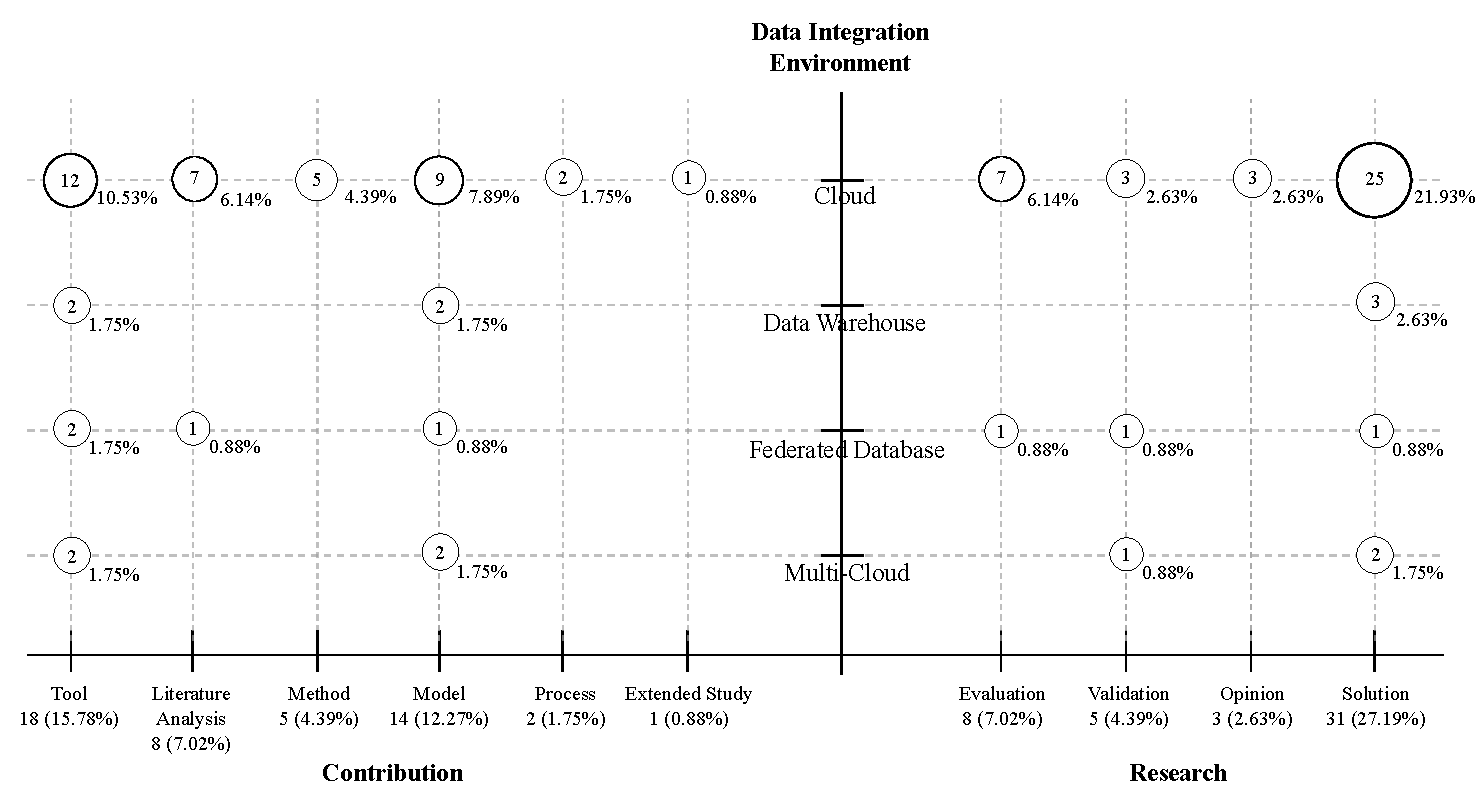
\includegraphics[width=0.86\textwidth]{figs/bubble-charts/DI-Environment-Contribution-Research.pdf}
\caption{Facets Data Integration Environment, Contribution and Research}\label{fig:facet2}
\end{figure}

Combining the facets data integration environment, contribution
and research it is possible to observe  the evolution of publications on data integration towards the cloud (Figure~\ref{fig:facet2}).  {\em Data warehouse} environments are the most common architecture. This can be explained by the increase of scientific  and industrial applications needing to build integrated  data sets for performing analysis and decision making tasks. The proposals are delivered as {\em models}  (14  papers - 12.27\%)  and {\em tools} (18
papers - 15.78\%)  used for facilitating data integration, mostly done in the {\em cloud}.  The most popular deployment environment of recent papers is the {\em cloud}. Given the importance and crucial need of data integration  most papers present concrete solutions as algorithms, methods and systems (31 papers - 27.19\%).

%Analyzing the figure is also possible to observe that Solution (31 appearances -
%27.19\%) is the type of research most proposed, followed by Evaluation (8
%appearances - 7.02\%), Validation (5 appearances - 4.39\%) and Opinion (3
%appearances - 2.63\%).


% As cloud becomes more centered in tecnological infraestructure, the
%challenge of integrating data on the cloud rises as well. 

%The contributions are diverse in respect of \textit{data integration} on the cloud environment. 
%There are many contributions based \textit{tool} solutions,
%which is the most frequent considering the analyzed studies. The
%proposed \textit{tools} used to assist the integration of data in the cloud.
%The new proposals for models and methods are quite frequent. So, resembling the
%use of SLA in the cloud, proposed solutions that consider data integration and
%cloud go in the same direction, new models, methods and tools. The combined
%analysis of Figures \ref{fig:facet2} and \ref{fig:facet4} answer this question,
%as we present following.


%A few other studies do literature review comparing work and presenting
%gaps in relation to these two areas. Considering Figure \ref{fig:facet2}, you
%can verify that most research types presented are new solutions. Others few show validation
%and evaluation ana;lysis of existing proposals.     


%Looking to the Figure ~\ref{fig:facet2} it is possible to identify that Tool  and Model are the mainly type
%of contribution developed, followed by Literature Analysis (8 appearances -
%7.02\%), Method (5 appearances - 4.39\%) Process (2 appearances - 1.75\%) and
%Extended Study (1 appearance - 0.88\%).
%Analyzing the figure is also possible to observe that Solution (31 appearances -
%27.19\%) is the type of research most proposed, followed by Evaluation (8
%appearances - 7.02\%), Validation (5 appearances - 4.39\%) and Opinion (3
%appearances - 2.63\%).
  
%  . .  .  . .  .  . .  .  . .  .  . .  .  . .  .  . .  .  . .  .  . .  .  . .  .  . .  .  . .  .  . .  .  . .  .  . .  .  . .  .  . .  .  . .  .  . .  .  . .  .  . .  .  . .  .
\textbf{\textit{RQ3:  In which way and in which context has data integration been linked to QoS measures in the literature?}}
%  . .  .  . .  .  . .  .  . .  .  . .  .  . .  .  . .  .  . .  .  . .  .  . .  .  . .  .  . .  .  . .  .  . .  .  . .  .  . .  .  . .  .  . .  .  . .  .  . .  .  . .  .  . .  .
\begin{figure}[!h]
\centering
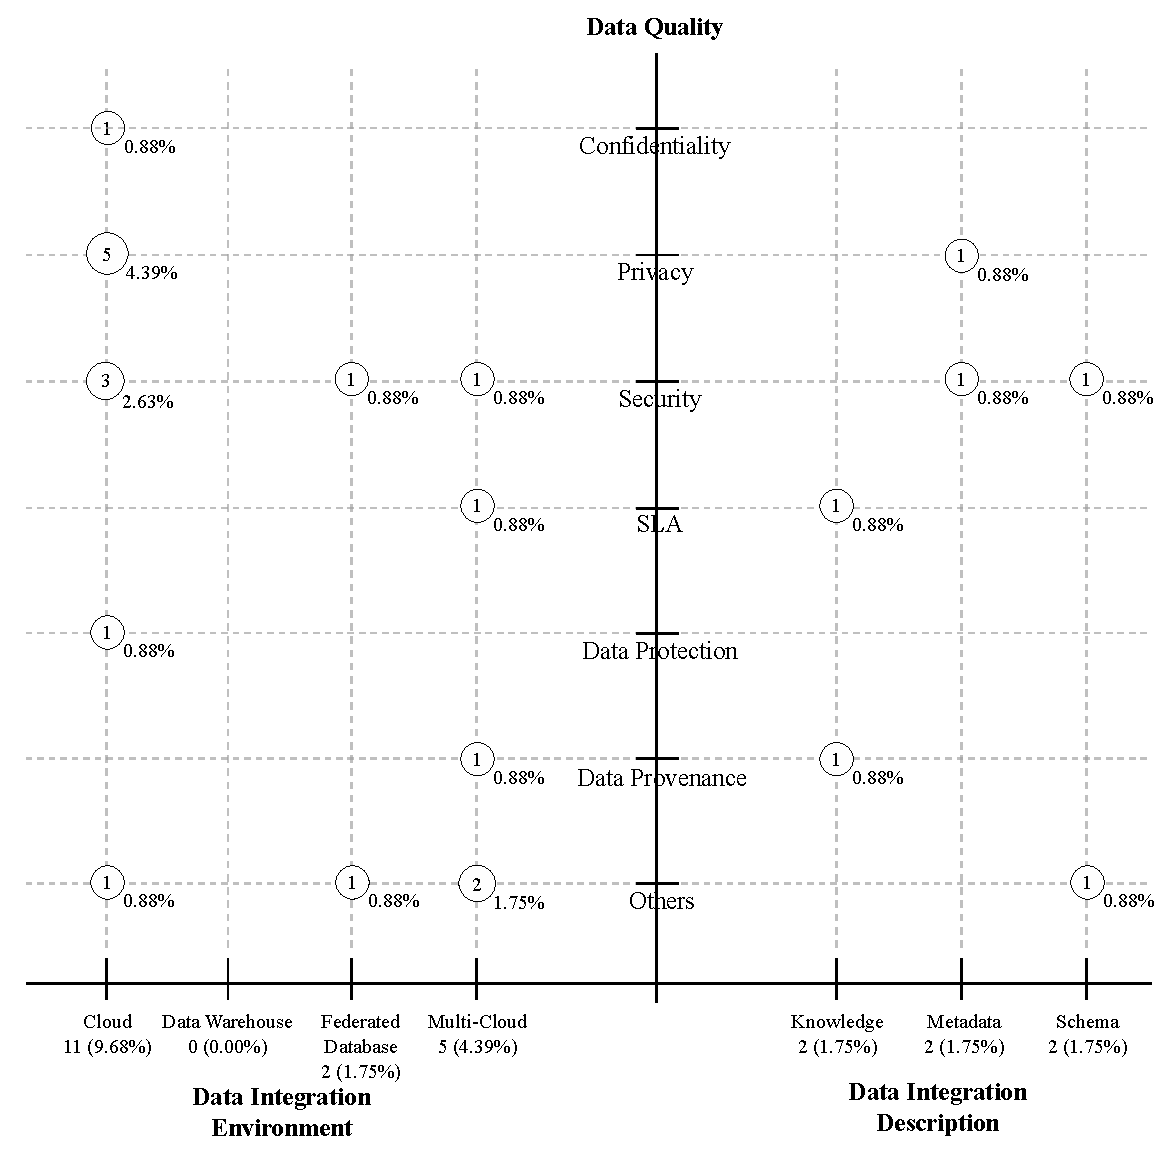
\includegraphics[width=0.85\textwidth]{figs/bubble-charts/Data-Quality-DI.pdf}
\caption{Facets Data Quality, Data Integration Environment and Data Integration Description}\label{fig:facet4}
\end{figure}

We answered RQ3 by combining the facet {\em data quality} with the facets {\em data integration environment} and {\em data integration description}
(Figure~\ref{fig:facet4}).  Data integration and QoS measures are associated within environments like cloud  (9.68\%) and multi-cloud (4.39\%).

According to our quantitative analysis we observe that QoS has started to be
considered for integrating data. 
%Papers 
%Yet, the type of measures and properties are still diverse. 
%They 
%address measures related to the conditions in which data are
%accessed like security and privacy.
 The cloud is becoming a popular environment to
perform data integration in which security issues are most frequently addressed.
We identify a promising research area concerning the need of studying SLA which
is currently addressed  for the cloud as a whole \cite{PedrinaciCL14} but that
needs to be specialized for data integration aspects. Therefore, it is important
to identify the measures that characterize the quality of data and  the
quality measures associated to different phases of data integration. These phases include selecting
data services, retrieving data, integrating and correlating them and building a
query result that can be eventually stored and that must be delivered. The data integration phases are implemented by greedy algorithms and generate intermediate data that
can be stored for further use. Therefore they consume storage, computing,
processing and communication resources that have an associated economic cost. These resources 
 must ensure some QoS guarantees to data consumers. This problem seems to be
open in the domain, and we believe that it must be part of  a new vision of data
integration. We believe that it is possible to add and enhance the quality of
data integration by including SLAs.                   

% \textit{Security} and \textit{privacy} the QoS measures that are most discussed together with data integration
 %(5 papers - 4.39\%). 
%The figure also shows that SLA has not been widely used in order to address data integration solutions
%(1 appearance) which reinforces our main objective of integrate SLA, data integration and multi-cloud 
%environments. 
%Analyzing the figure is also possible to observe that the most deployed data integration environment is 
%the cloud (9.68\%) followed by multi-cloud (4.39\%), federated databases (1.75\%) and data warehouse (0.00\%).
%The data integration description dimensions had the same percentage for schema, knowledge and metadata (2 appearance - 1.75\%)

% Most data integration environment consider cloud for solution. 
% 
% The type of contribution envolving data integration most often are
% \textit{tools} and \textit{models}, respectively. Some few others focus on the
% proposition of \textit{methods} or \textit{process}. 
